% GNUPLOT: LaTeX picture with Postscript
\begingroup
  \makeatletter
  \providecommand\color[2][]{%
    \GenericError{(gnuplot) \space\space\space\@spaces}{%
      Package color not loaded in conjunction with
      terminal option `colourtext'%
    }{See the gnuplot documentation for explanation.%
    }{Either use 'blacktext' in gnuplot or load the package
      color.sty in LaTeX.}%
    \renewcommand\color[2][]{}%
  }%
  \providecommand\includegraphics[2][]{%
    \GenericError{(gnuplot) \space\space\space\@spaces}{%
      Package graphicx or graphics not loaded%
    }{See the gnuplot documentation for explanation.%
    }{The gnuplot epslatex terminal needs graphicx.sty or graphics.sty.}%
    \renewcommand\includegraphics[2][]{}%
  }%
  \providecommand\rotatebox[2]{#2}%
  \@ifundefined{ifGPcolor}{%
    \newif\ifGPcolor
    \GPcolortrue
  }{}%
  \@ifundefined{ifGPblacktext}{%
    \newif\ifGPblacktext
    \GPblacktextfalse
  }{}%
  % define a \g@addto@macro without @ in the name:
  \let\gplgaddtomacro\g@addto@macro
  % define empty templates for all commands taking text:
  \gdef\gplbacktext{}%
  \gdef\gplfronttext{}%
  \makeatother
  \ifGPblacktext
    % no textcolor at all
    \def\colorrgb#1{}%
    \def\colorgray#1{}%
  \else
    % gray or color?
    \ifGPcolor
      \def\colorrgb#1{\color[rgb]{#1}}%
      \def\colorgray#1{\color[gray]{#1}}%
      \expandafter\def\csname LTw\endcsname{\color{white}}%
      \expandafter\def\csname LTb\endcsname{\color{black}}%
      \expandafter\def\csname LTa\endcsname{\color{black}}%
      \expandafter\def\csname LT0\endcsname{\color[rgb]{1,0,0}}%
      \expandafter\def\csname LT1\endcsname{\color[rgb]{0,1,0}}%
      \expandafter\def\csname LT2\endcsname{\color[rgb]{0,0,1}}%
      \expandafter\def\csname LT3\endcsname{\color[rgb]{1,0,1}}%
      \expandafter\def\csname LT4\endcsname{\color[rgb]{0,1,1}}%
      \expandafter\def\csname LT5\endcsname{\color[rgb]{1,1,0}}%
      \expandafter\def\csname LT6\endcsname{\color[rgb]{0,0,0}}%
      \expandafter\def\csname LT7\endcsname{\color[rgb]{1,0.3,0}}%
      \expandafter\def\csname LT8\endcsname{\color[rgb]{0.5,0.5,0.5}}%
    \else
      % gray
      \def\colorrgb#1{\color{black}}%
      \def\colorgray#1{\color[gray]{#1}}%
      \expandafter\def\csname LTw\endcsname{\color{white}}%
      \expandafter\def\csname LTb\endcsname{\color{black}}%
      \expandafter\def\csname LTa\endcsname{\color{black}}%
      \expandafter\def\csname LT0\endcsname{\color{black}}%
      \expandafter\def\csname LT1\endcsname{\color{black}}%
      \expandafter\def\csname LT2\endcsname{\color{black}}%
      \expandafter\def\csname LT3\endcsname{\color{black}}%
      \expandafter\def\csname LT4\endcsname{\color{black}}%
      \expandafter\def\csname LT5\endcsname{\color{black}}%
      \expandafter\def\csname LT6\endcsname{\color{black}}%
      \expandafter\def\csname LT7\endcsname{\color{black}}%
      \expandafter\def\csname LT8\endcsname{\color{black}}%
    \fi
  \fi
    \setlength{\unitlength}{0.0500bp}%
    \ifx\gptboxheight\undefined%
      \newlength{\gptboxheight}%
      \newlength{\gptboxwidth}%
      \newsavebox{\gptboxtext}%
    \fi%
    \setlength{\fboxrule}{0.5pt}%
    \setlength{\fboxsep}{1pt}%
\begin{picture}(14400.00,10080.00)%
    \gplgaddtomacro\gplbacktext{%
      \csname LTb\endcsname%
      \put(814,704){\makebox(0,0)[r]{\strut{}$0$}}%
      \put(814,2156){\makebox(0,0)[r]{\strut{}$0.5$}}%
      \put(814,3609){\makebox(0,0)[r]{\strut{}$1$}}%
      \put(814,5061){\makebox(0,0)[r]{\strut{}$1.5$}}%
      \put(814,6513){\makebox(0,0)[r]{\strut{}$2$}}%
      \put(814,7966){\makebox(0,0)[r]{\strut{}$2.5$}}%
      \put(814,9418){\makebox(0,0)[r]{\strut{}$3$}}%
      \put(946,484){\makebox(0,0){\strut{}$0$}}%
      \put(1599,484){\makebox(0,0){\strut{}$10$}}%
      \put(2252,484){\makebox(0,0){\strut{}$20$}}%
      \put(2904,484){\makebox(0,0){\strut{}$30$}}%
      \put(3557,484){\makebox(0,0){\strut{}$40$}}%
      \put(4210,484){\makebox(0,0){\strut{}$50$}}%
      \put(4863,484){\makebox(0,0){\strut{}$60$}}%
      \put(5516,484){\makebox(0,0){\strut{}$70$}}%
      \put(6168,484){\makebox(0,0){\strut{}$80$}}%
      \put(6821,484){\makebox(0,0){\strut{}$90$}}%
      \put(7474,484){\makebox(0,0){\strut{}$100$}}%
      \put(8127,484){\makebox(0,0){\strut{}$110$}}%
      \put(8780,484){\makebox(0,0){\strut{}$120$}}%
      \put(9432,484){\makebox(0,0){\strut{}$130$}}%
      \put(10085,484){\makebox(0,0){\strut{}$140$}}%
      \put(10738,484){\makebox(0,0){\strut{}$150$}}%
      \put(11391,484){\makebox(0,0){\strut{}$160$}}%
      \put(12044,484){\makebox(0,0){\strut{}$170$}}%
      \put(12696,484){\makebox(0,0){\strut{}$180$}}%
      \put(13349,484){\makebox(0,0){\strut{}$190$}}%
      \put(14002,484){\makebox(0,0){\strut{}$200$}}%
    }%
    \gplgaddtomacro\gplfronttext{%
      \csname LTb\endcsname%
      \put(176,5061){\rotatebox{-270}{\makebox(0,0){\Large Elevation (Kilometers)}}}%
      \put(7474,154){\makebox(0,0){\strut{}\vspace{-0.5in}{\Large Distance from QTH, in km}}}%
      \put(7474,9748){\makebox(0,0){\strut{}\vspace{0.5in}{\LARGE 4:3 Earth Propagation Diagram}}}%
    }%
    \gplbacktext
    \put(0,0){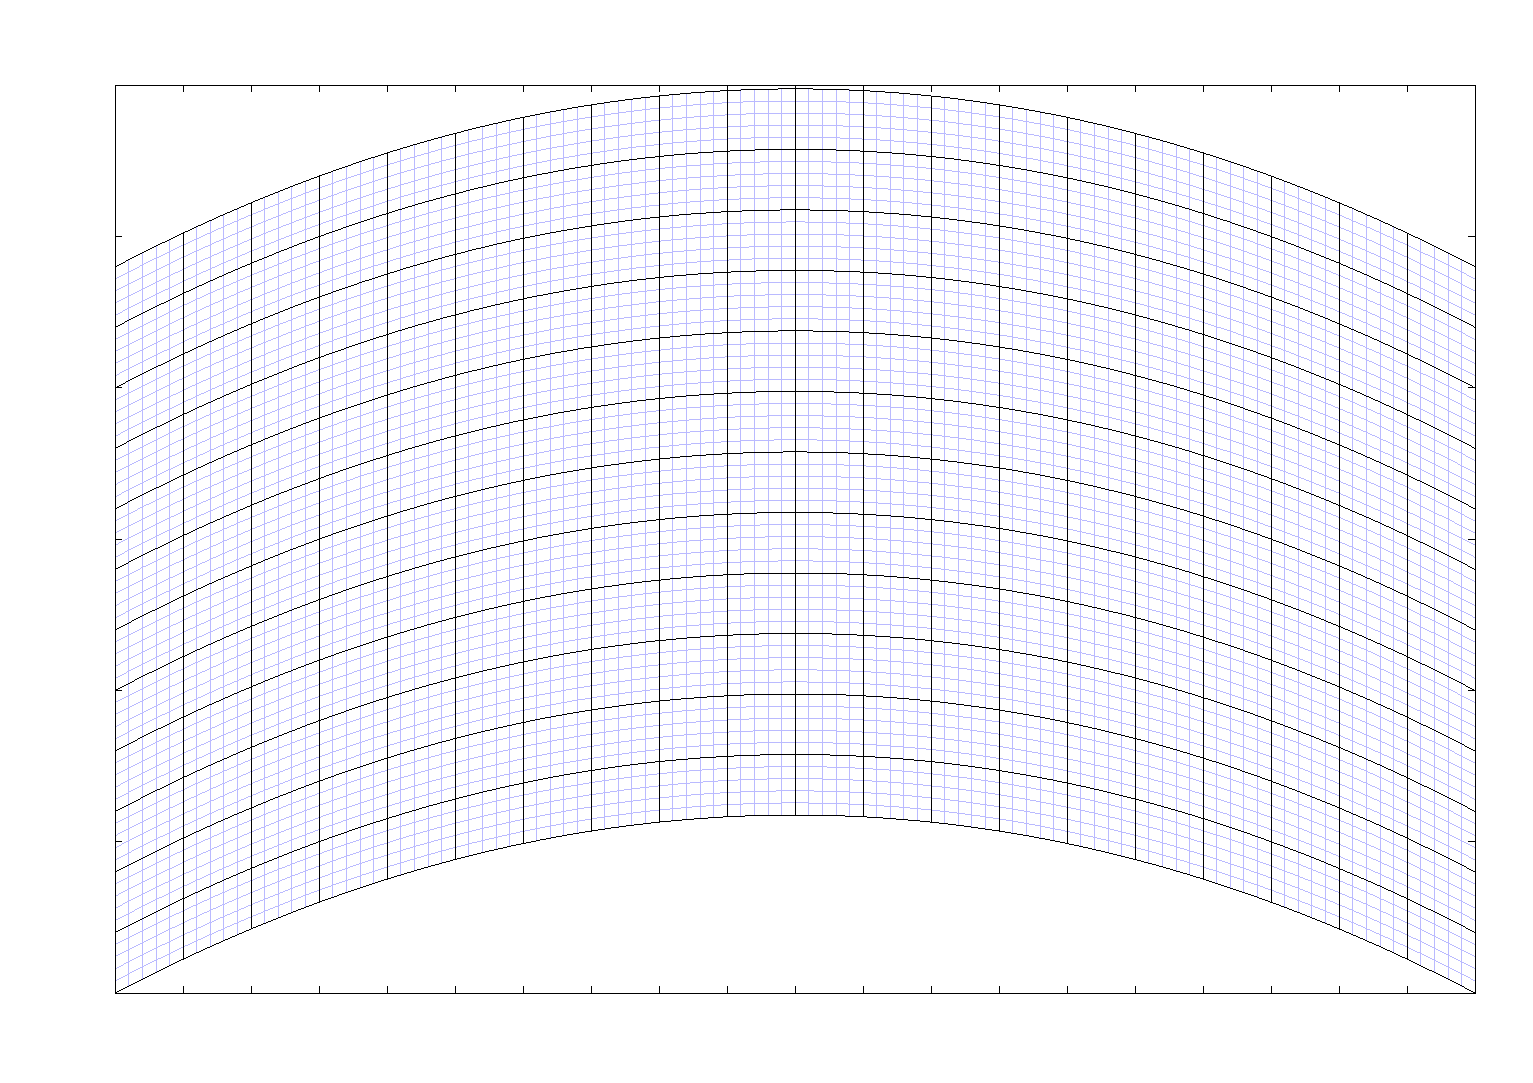
\includegraphics{inserteps}}%
    \gplfronttext
  \end{picture}%
\endgroup
